\documentclass{article}

\usepackage[a4paper,left=18mm,right=18mm,top=20mm,bottom=18mm]{geometry}
\usepackage[italian]{babel}

\usepackage{titling}
\usepackage{graphicx}
\usepackage{subcaption}
\usepackage{float}
 
\title{PDF con tutti i grafici UML}
\author{Nicolas Anselmi, David Guzman Piedrahita and Marco Vinciguerra}

\begin{document}
\maketitle
\section{Use case diagram}

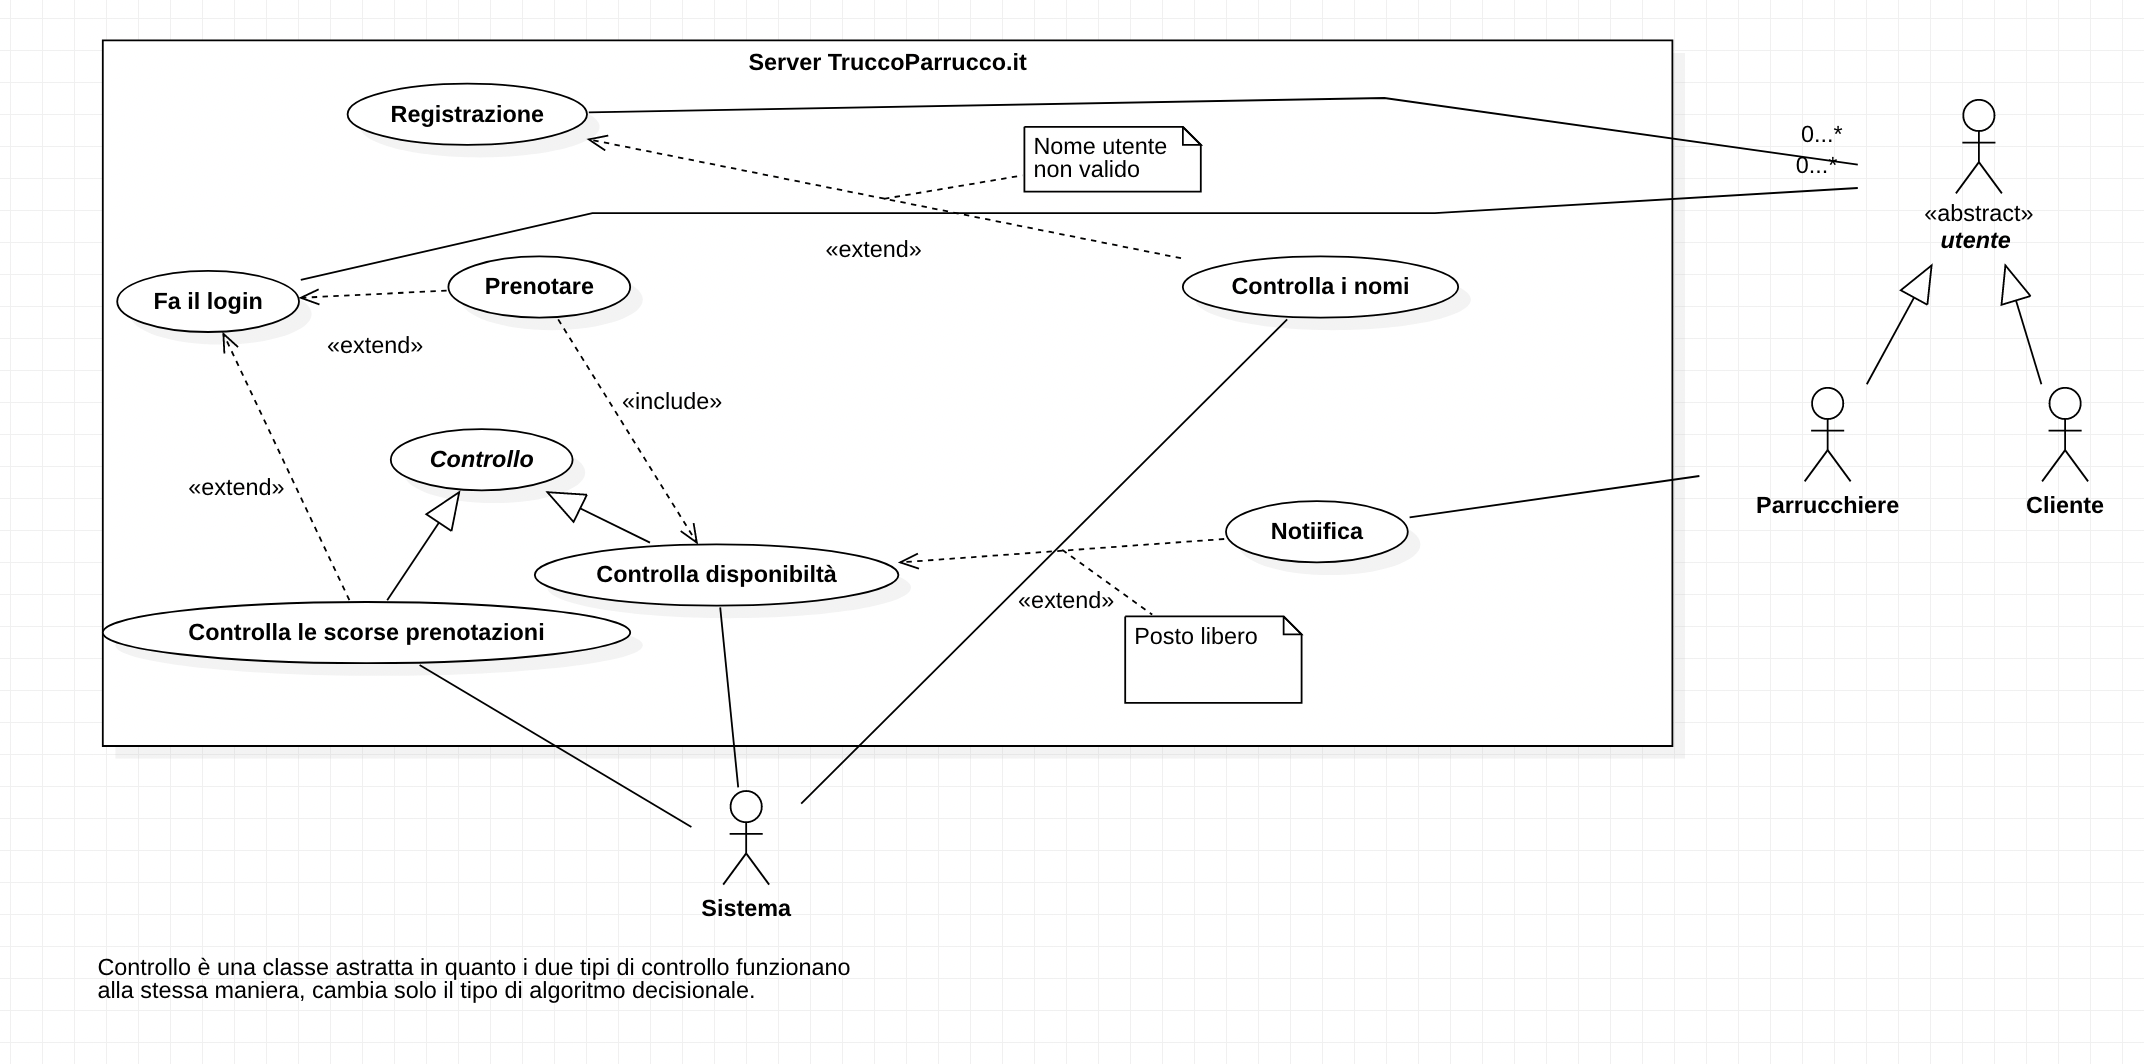
\includegraphics[scale = 0.5]{Immagini/UseCaseDiagram.png}

\section{Class diagram}
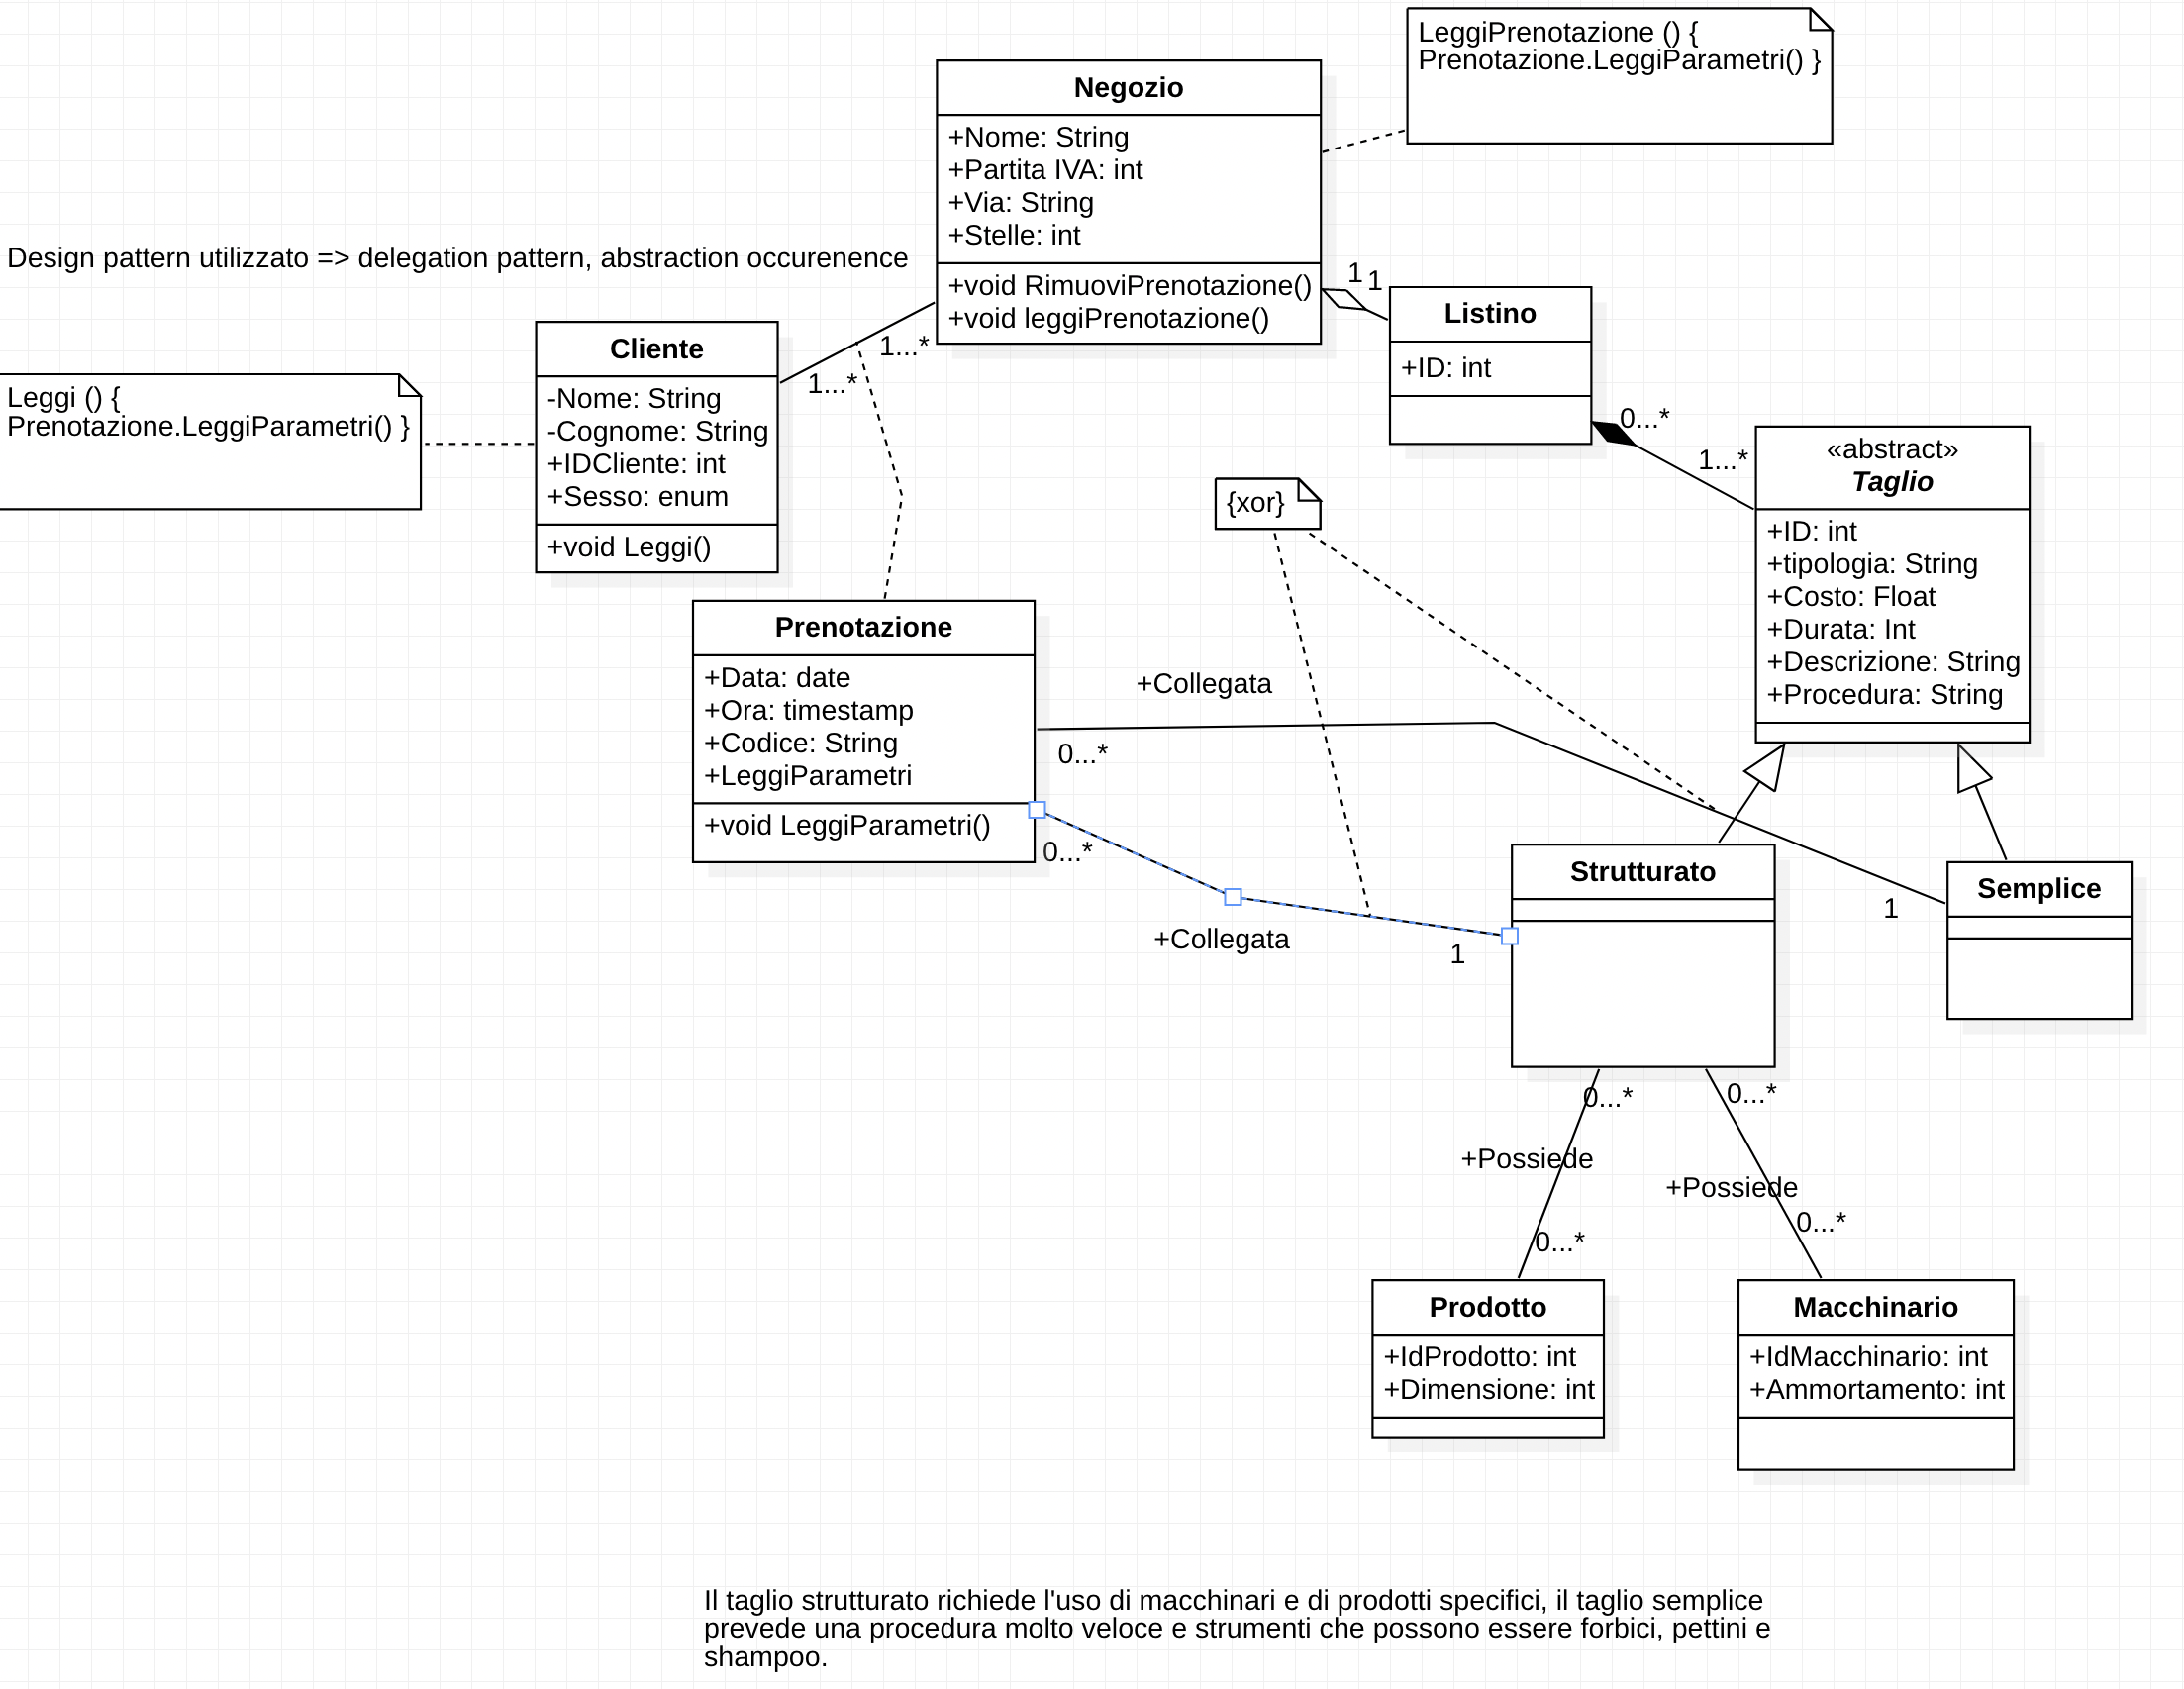
\includegraphics[scale = 0.5]{Immagini/ClassDiagram.png}

\section{State machine diagram}
\subsection{State machine diagram che rappresenta la richiesta}
TOODO $\rightarrow$ aggiungere questo diagramma

\subsection{State machine diagram del parrucchiere}
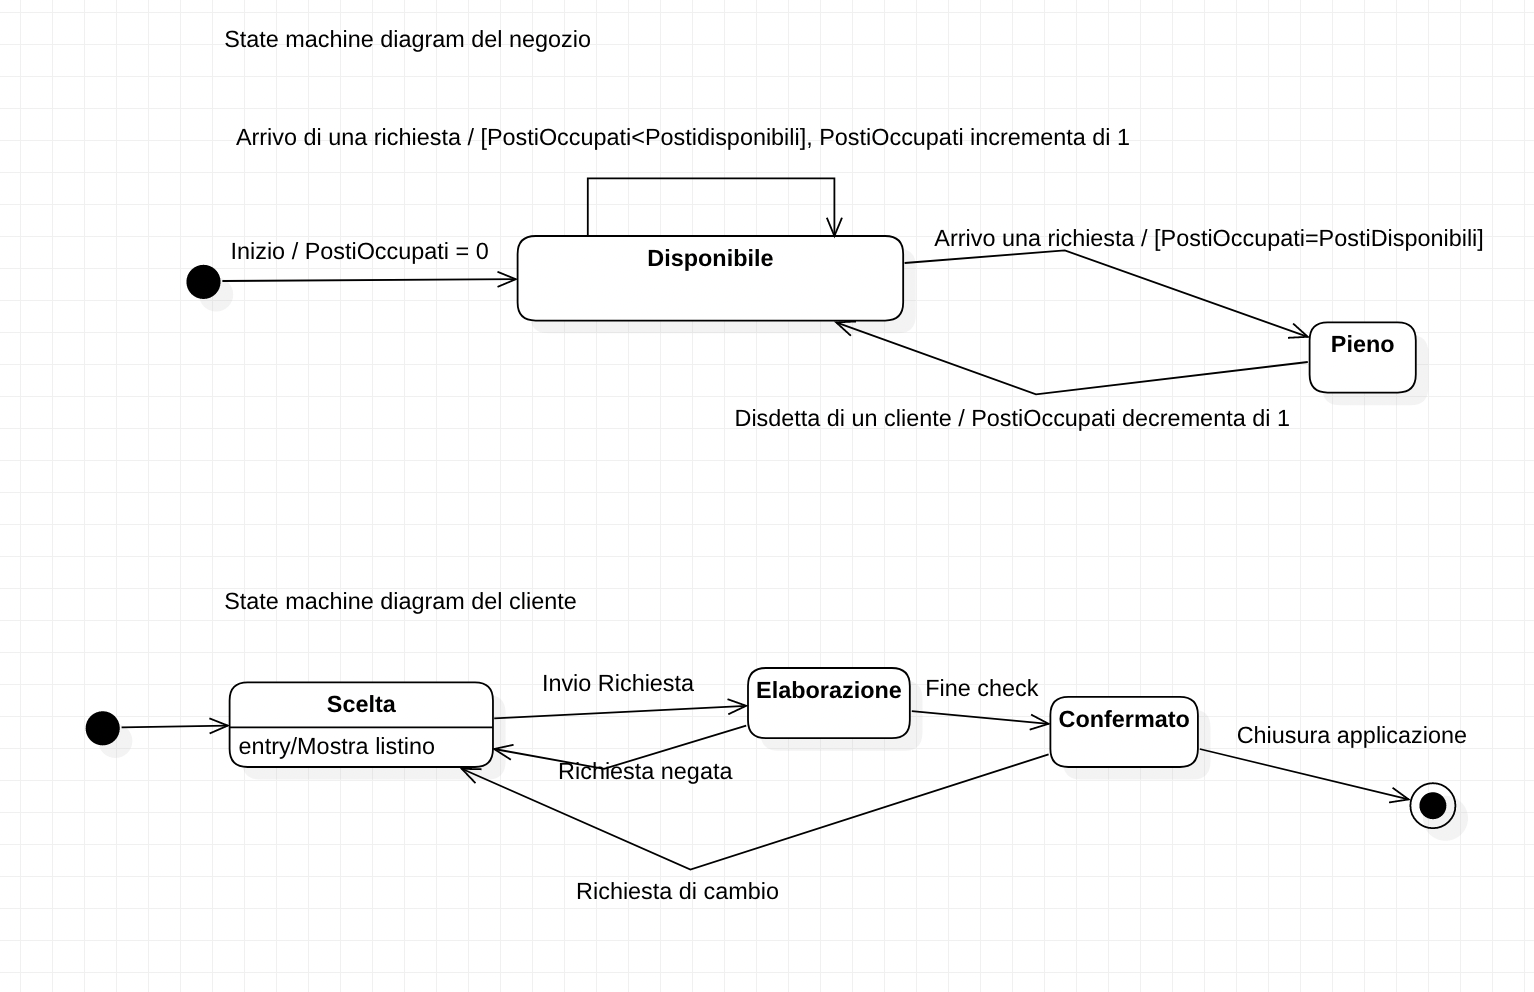
\includegraphics[scale = 0.5]{Immagini/StateMachineDiagram.png}

\section{Sequence diagram}
\subsection{Sequence diagram del login}
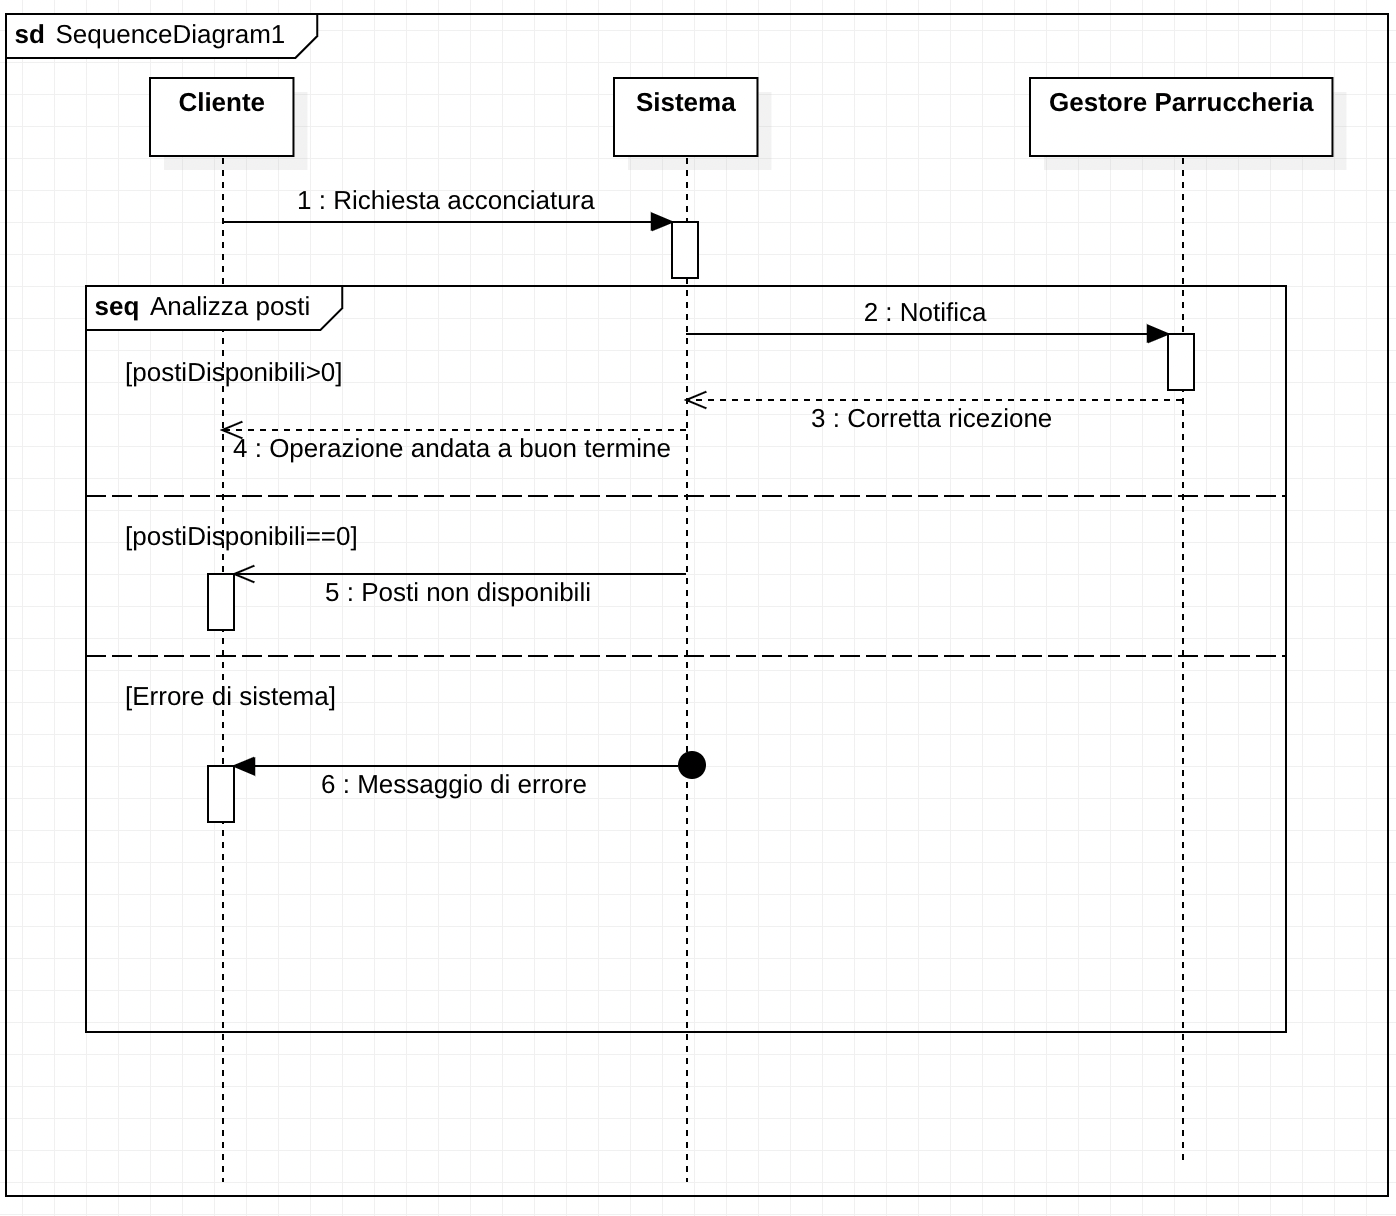
\includegraphics[scale = 0.5]{Immagini/Sequence diagram Login.png}
\subsection{Sequence diagram della registrazione}
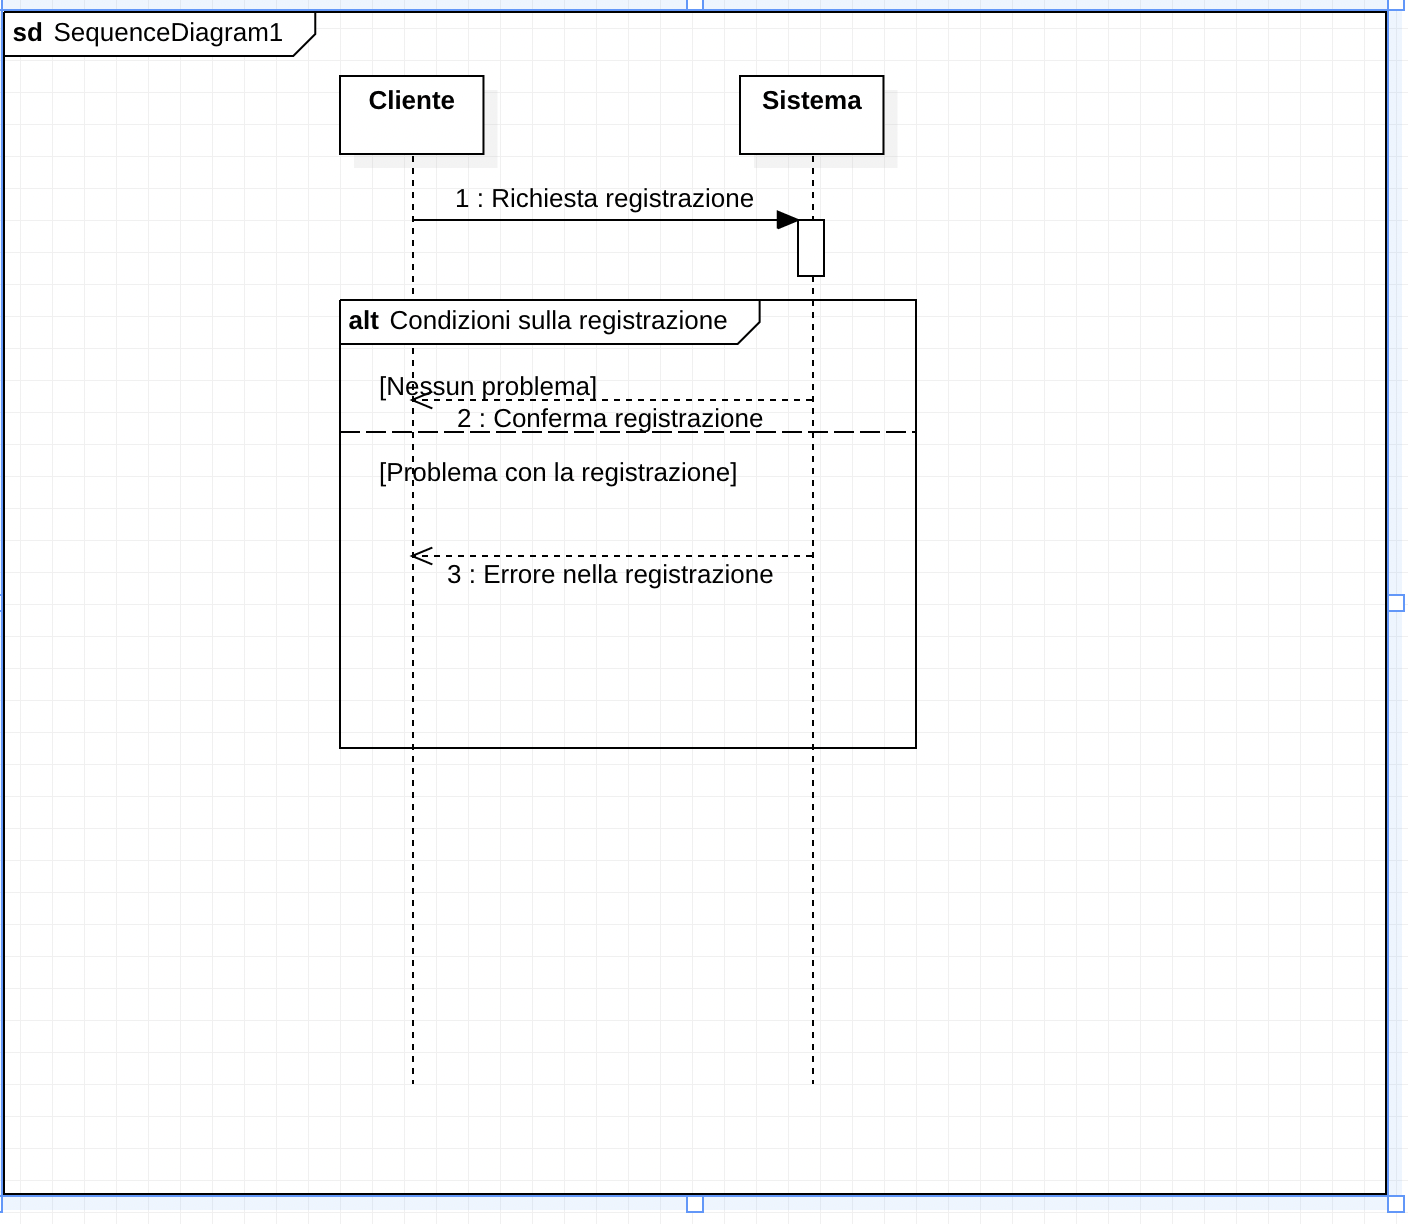
\includegraphics[scale = 0.5]{Immagini/Sequence diagram registrazione.png}

\section{Activity diagram}
\subsection{Granularità alta}
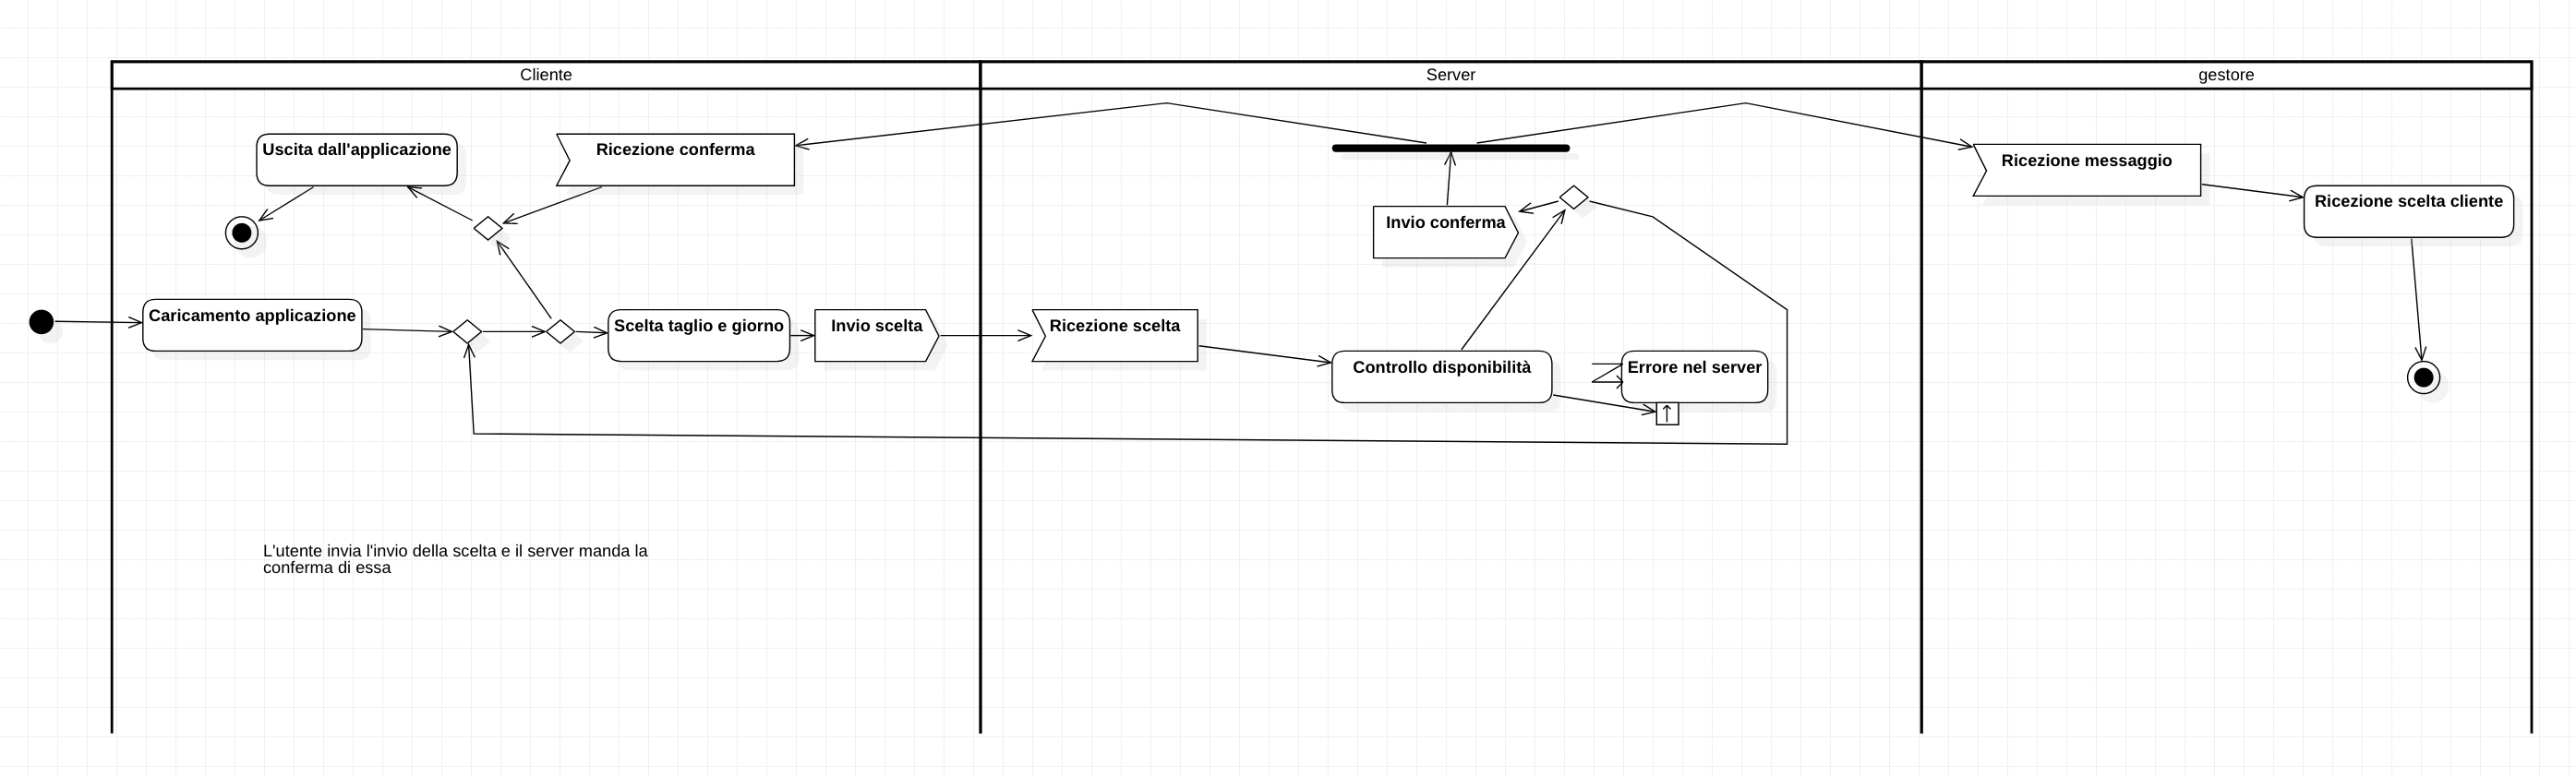
\includegraphics[scale = 0.35]{Immagini/ActivityDiagram1.png}

\subsection{Granularità bassa}
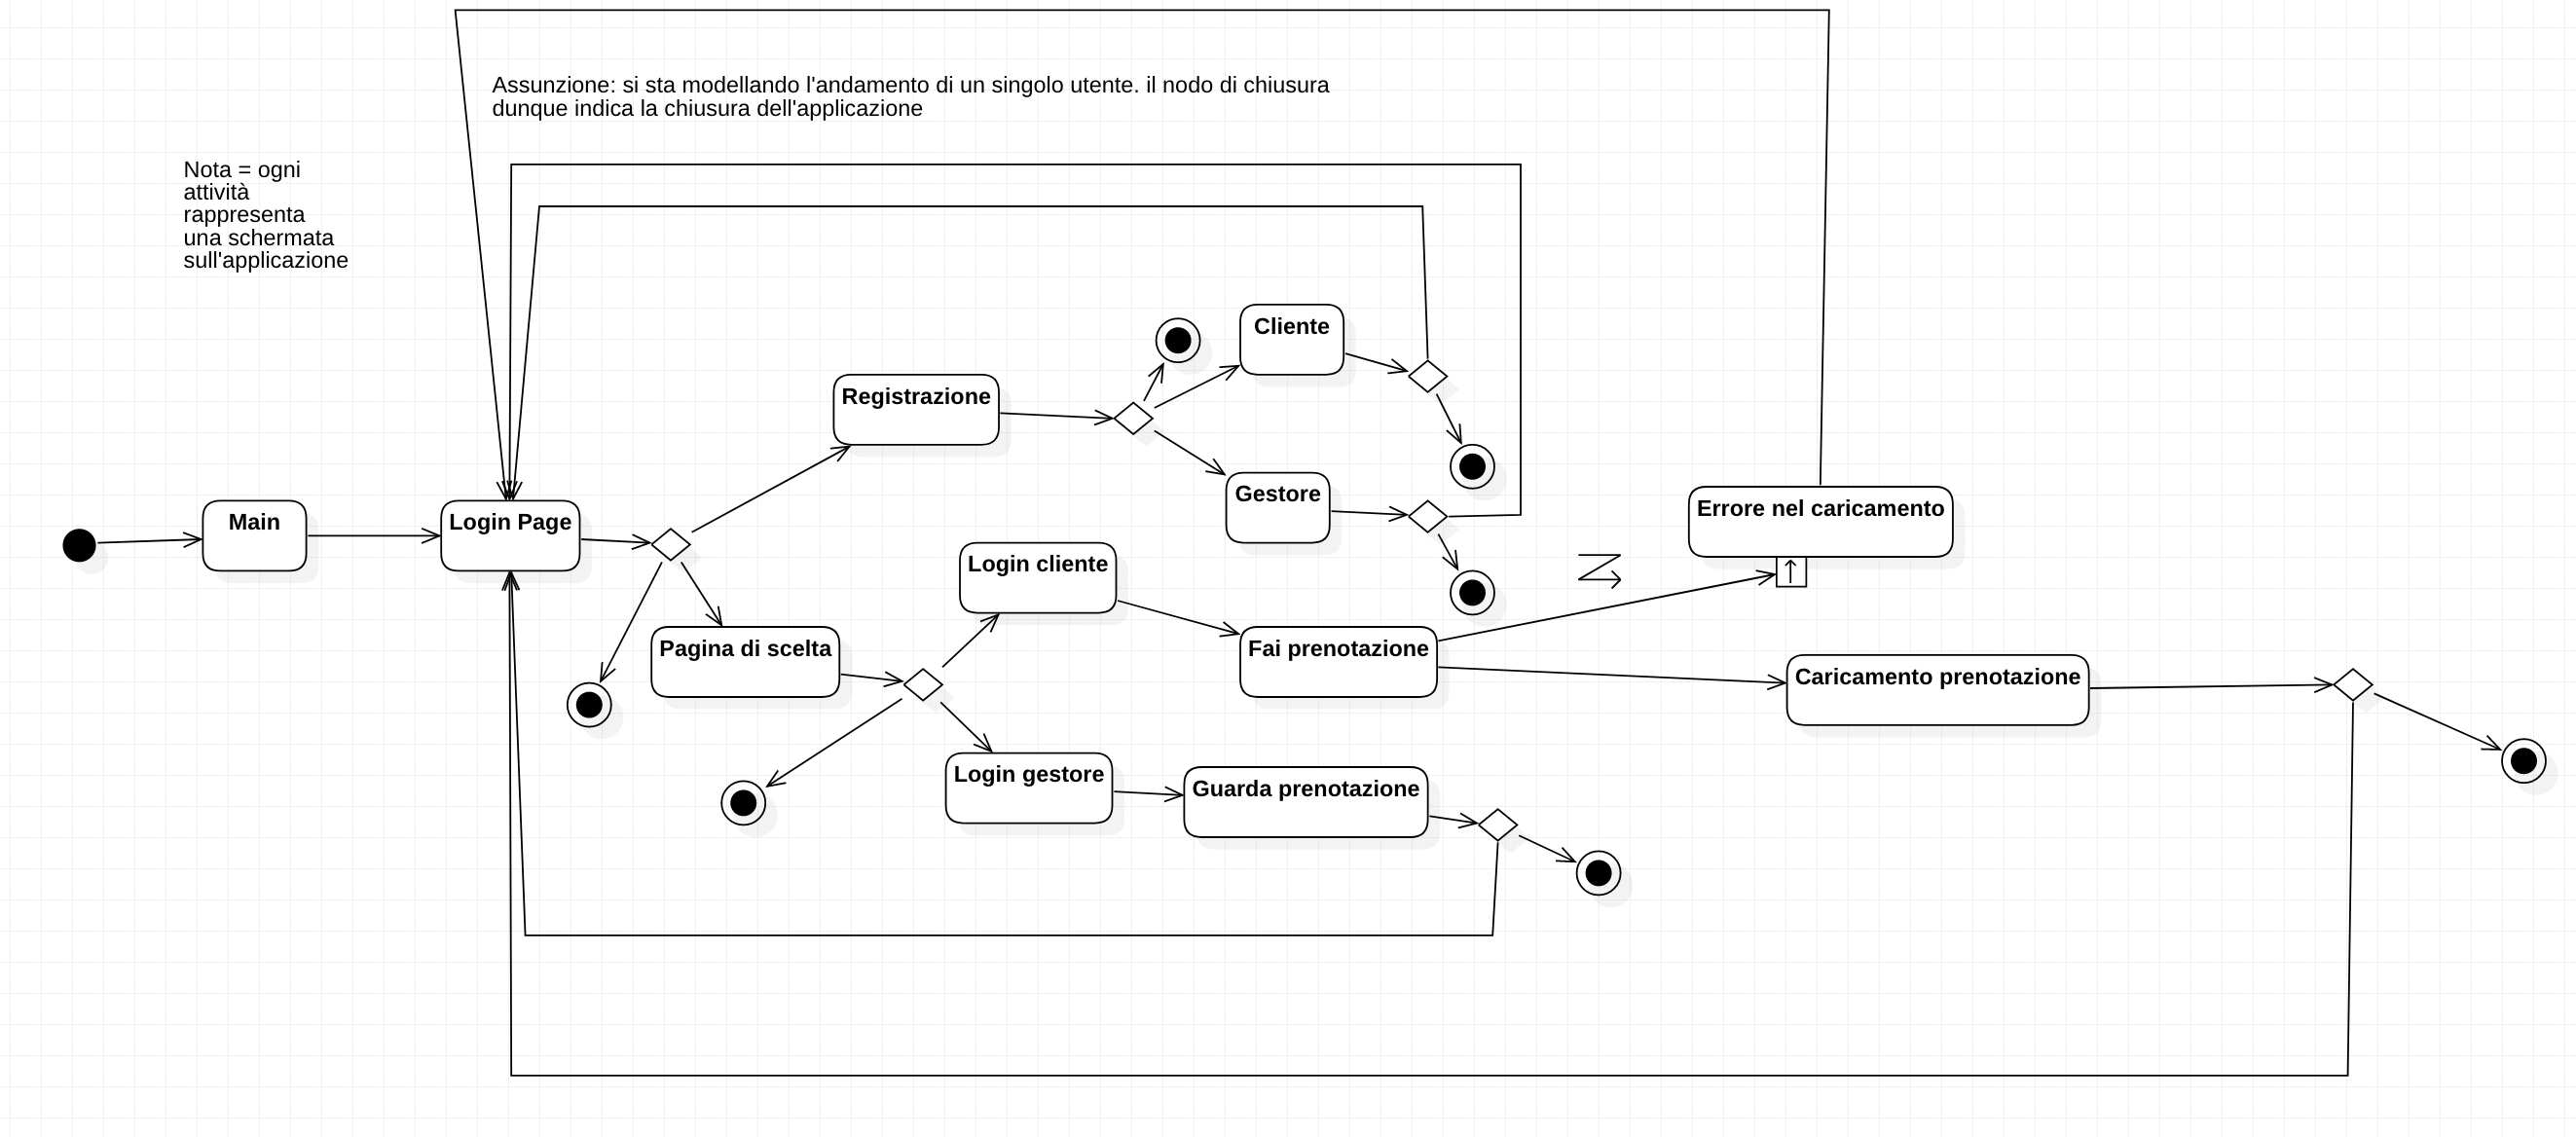
\includegraphics[scale = 0.4]{Immagini/ActivityDiagram2.png}
\end{document}
